
\documentclass[twocolumn, journal]{IEEEtran}

\usepackage{cite}
\usepackage{amsmath,amssymb,amsfonts}
\usepackage{algorithmic}
\usepackage{graphicx}
\usepackage{textcomp}
\usepackage{xcolor}
\usepackage{booktabs}
\usepackage{microtype}
\usepackage{url}
\usepackage{tikz}
\usepackage{pgfplots}
\pgfplotsset{compat=1.18}
\usetikzlibrary{arrows.meta, positioning, shapes.geometric, fit, backgrounds, calc}
\usepackage{subfig}
\usepackage[hidelinks]{hyperref}

\begin{document}

\title{One Bit is All You Need to Diffuse}

\author{
\IEEEauthorblockN{Nihal Gazi}
\IEEEauthorblockA{Dept. CSE AI \& ML, IEM\\nihlg2006@gmail.com}
\and
\IEEEauthorblockN{Ayushman Bhattacharya}
\IEEEauthorblockA{MyceliAI A\"U\\ayushman@myceli.ai}
\and
\IEEEauthorblockN{Aditya K. Biswas}
\IEEEauthorblockA{Dept. CSE \& Business Systems, IEM\\adityakb@gmail.com}
\and 
\IEEEauthorblockN{Saubhagya Kunti}
\IEEEauthorblockA{Dept. CSE \& Business Systems, IEM\\sauabhagya.kunti@gmail.com}
\and
\IEEEauthorblockN{Aihik Basu}
\IEEEauthorblockA{Dept. CSE Engineering, IEM\\aihik.basu@gmail.com}
}

\maketitle

\begin{abstract}
The memory footprint and arithmetic cost of floating-point operations remain the
principal obstacles to running generative diffusion models on edge hardware. Reducing
weights all the way down to a single bit would, in theory, resolve both issues---yet
the prevailing view in the literature holds that such aggressive quantization destroys
the generative manifold beyond recovery. This paper argues otherwise. We show that the
collapse attributed to 1-bit precision is actually an artifact of the
Post-Training Quantization (PTQ) workflow, not a fundamental limit of binary
representation. To substantiate this claim we propose \textbf{Native Binarization}, a
training regime in which diffusion models are built from the ground up with 1-bit
weights, mean-centered scaling, and pre-activation block ordering. Two properties
underpin the approach: \emph{structural dominance}, whereby centered binarization
retains the dominant directional geometry of each weight tensor, and
\emph{topological stability}, whereby the binary network preserves manifold coherence
across the entire training trajectory. In a controlled W1A16 ablation---binary weights
paired with full-precision activations---PTQ yields an FID of~191.94 and a legibility
of only~64.92\%, whereas our natively trained counterpart reaches an FID of~24.24 with
89.45\% legibility, marginally outperforming even the FP16 baseline (FID~29.60,
legibility~90.79\%). No teacher network or distillation step is involved at any point.
The resulting architecture offers a 32$\times$ reduction in weight storage and a
58$\times$ speed-up in binary operations while preserving semantic quality. As far as
we are aware, no prior work has demonstrated that a binary diffusion model trained
entirely from scratch can match full-precision generation quality.
\end{abstract}

\noindent\textbf{Keywords:} 1-Bit Quantization, Diffusion Models, Generative AI, Model Compression, Topology,
ResUNet, Edge AI, Structural Dominance, Binary Neural Networks

\section{Introduction}

Denoising diffusion models have rapidly become one of the most capable families of
generative models in modern machine learning. Denoising Diffusion Probabilistic Models
(DDPMs)~\cite{ho2020ddpm} routinely produce images of remarkable quality across a range
of domains, but their reliance on floating-point matrix arithmetic ties them to
power-hungry GPUs and server-grade accelerators. With growing demand for on-device
intelligence---in mobile phones, wearables, and IoT sensors---this dependence poses a
real problem. Executing the 1{,}000 sequential denoising steps that a typical DDPM
requires is simply not feasible on an FP16 edge processor today.

One appealing remedy is to push weight precision to its absolute minimum: a single bit.
Compressing 16- or 32-bit floating-point parameters into $\{-1,+1\}$ values would
replace costly multiply-accumulate (MAC) instructions with XNOR-popcount logic, cutting
both memory and energy consumption by orders of magnitude. The catch, according to
current research, is that such extreme compression fundamentally breaks diffusion
models. The most recent investigation of this question---Binarized Diffusion Model
(BiDM)~\cite{bidm2024}, presented at NeurIPS 2024---reported that binarization
collapses the generative manifold entirely, and that an elaborate distillation pipeline
from a full-precision teacher is the only viable path to recovery.

Our work takes issue with that conclusion. The manifold destruction documented in
earlier studies, we argue, stems not from any intrinsic limitation of 1-bit
arithmetic but from the way binarization has been applied---namely, through
\textbf{Post-Training Quantization (PTQ)}. PTQ frames binarization as a
\emph{compression task}: a carefully trained FP16 model has its weights snapped to
binary values after the fact. This ``train first, binarize later'' pipeline strips
away the finely tuned magnitude relationships that encode the learned score field,
leaving behind severe structural damage and sharply reduced generation quality.

We take a fundamentally different approach.  \textbf{Native Binarization} treats the
problem as one of \emph{representation} rather than compression. Instead of converting
a floating-point model, we train a diffusion network from random initialization under
binary weight constraints from the very first gradient step. Two design choices make
this feasible: (1)~\textbf{mean-centered weight scaling}, which preserves what we call
\emph{structural dominance}---the dominant directional structure of each filter is
retained after binarization---and (2)~\textbf{pre-activation residual ordering}
(BN $\to$ Act $\to$ Conv), which maintains \emph{topological stability} by keeping
gradient flow through the sign function well-conditioned at every stage of training.

We validate the idea with a tightly controlled W1A16 hardware ablation: activations are
held at FP16 while only the weight binarization method varies. Under PTQ the model
degrades sharply (FID:~191.94, legibility:~64.92\%). The natively trained binary model,
by contrast, reaches FID~24.24 with 89.45\% legibility---on par with, and slightly
better than, the FP16 baseline (FID~29.60, legibility~90.79\%). In practical terms,
more than 96\% of the parametric precision is eliminated, yielding a 32$\times$
reduction in weight storage and a 58$\times$ speed-up in binary operations, all without
meaningful loss of generative quality.

\textbf{Contributions.} The main contributions of this work are as follows:
\begin{itemize}
  \item We provide, to our knowledge, the first evidence that a 1-bit diffusion model
    can be trained from scratch---with no full-precision teacher, no knowledge
    distillation, and no pre-trained starting point---while matching the FP16 baseline
    in generation quality. This result directly contradicts the position, underscored by
    BiDM~\cite{bidm2024}, that distillation from a teacher is indispensable for binary
    diffusion.
  \item We articulate and formalize two guiding principles---\textbf{structural
    dominance} (directional weight geometry is preserved through centered binarization)
    and \textbf{topological stability} (manifold integrity is maintained via
    pre-activation ordering)---that together explain why native training works at 1-bit
    where PTQ severely degrades.
  \item We construct a controlled \textbf{W1A16 hardware ablation} that decouples the
    effect of weight binarization from activation quantization noise, enabling the first
    head-to-head comparison of PTQ and native training at the 1-bit boundary. The
    design lets us attribute observed quality loss specifically to the PTQ methodology,
    not to the bit-width itself.
  \item We propose the \textbf{Legibility Score}, a per-sample confidence metric that
    complements FID by capturing whether each generated image commits to a recognizable
    class. We show its value for separating distributional fidelity from per-sample
    structural validity across the FP16, W1A16, and W1A1 precision regimes.
\end{itemize}


\section{Related Work}

\subsection{Diffusion Models and Edge Deployment}

At a high level, a DDPM~\cite{ho2020ddpm} corrupts training images with Gaussian noise
over $T$ forward steps and then trains a network $f_\theta$ to reverse this corruption.
The loss function takes the form:
\begin{equation}
  \mathcal{L} = \mathbb{E}_{x_0,\varepsilon,t}\!\left[
    \left\|\varepsilon - f_\theta\!\left(\sqrt{\bar\alpha_t}\,x_0 +
    \sqrt{1-\bar\alpha_t}\,\varepsilon,\;t\right)\right\|^2\right]
  \label{eq:ddpm}
\end{equation}
with $\bar\alpha_t = \prod_{i=1}^{t}(1-\beta_i)$. Follow-up work---including
DDIM~\cite{song2020ddim}, Latent Diffusion~\cite{rombach2022ldm}, and
SDXL~\cite{podell2023sdxl}---has pushed image quality substantially further, yet every
variant inherits the same inference bottleneck: hundreds or thousands of sequential
forward passes through the denoising network. Attempts to bring diffusion models to edge
devices have largely targeted sampling speed (e.g.\ progressive
distillation~\cite{salimans2022progressive}) or network pruning, but neither strategy
tackles the underlying cost of floating-point arithmetic itself.

\subsection{Post-Training Quantization and Its Limits}

The idea behind PTQ is straightforward: take an already-trained model and re-map its
floating-point parameters to a lower bit-width, skipping any retraining.
Q-Diffusion~\cite{li2023qdiffusion} and PTQD~\cite{he2023ptqd} showed that diffusion
models can be quantized to 4 or 8 bits with tolerable quality loss. Later methods such
as EfficientDiffusion and TDQ added timestep-aware calibration, recognizing that
activation statistics in diffusion networks shift considerably from one denoising step
to the next and that a single static scale is therefore sub-optimal.

The trouble is that PTQ quality falls off a cliff as bit-width shrinks. At the 1-bit
extreme, quantization error dwarfs the weight magnitudes, and the pre-trained solution
surface is effectively destroyed. Our own experiments bear this out: a W1A16 model
obtained by PTQ records an FID of~191.94 and only~64.92\% legibility, whereas the same
architecture trained natively under binary constraints achieves FID~24.24 and 89.45\%
legibility.

\subsection{The 1-Bit Binarization Bottleneck}

In a Binary Neural Network
(BNN)~\cite{hubara2016bnn,rastegari2016xnornet}, both weights and activations are
restricted to $\{-1,+1\}$, turning multiply-accumulate arithmetic into XNOR-popcount
logic. XNOR-Net popularized per-channel scale factors
($\alpha = \text{mean}|W|$) as a way to narrow the quantization gap, and the
Straight-Through Estimator (STE)~\cite{bengio2013ste} made it possible to back-propagate
through the non-differentiable sign function, opening the door to end-to-end training.
BNNs have proven effective for discriminative tasks such as image
classification~\cite{liu2020reactnet,martinez2020training}, but generative
modelling---where the network must faithfully capture the full data distribution instead
of merely assigning labels---has seen very little exploration at the binary level.

The first attempt to fully binarize a diffusion model is
BiDM~\cite{bidm2024}, which operates at W1A1 precision and reports FID~22.74 on
LSUN-Bedrooms at $256{\times}256$ resolution. BiDM combines a Timestep-friendly Binary
Structure (TBS) with Space Patched Distillation (SPD), achieving a 28.0$\times$
reduction in storage and 52.7$\times$ fewer operations. A key limitation, however, is
that BiDM depends on a pre-trained full-precision teacher for the distillation
stage---a dependency that our method eliminates completely.

\subsection{Pre-Activation Residual Networks}

He et al.~\cite{he2016preact} demonstrated that moving batch normalization and the
non-linearity ahead of the convolution (BN $\to$ Act $\to$ Conv) yields better gradient
propagation in deep residual networks. For BNNs the benefits are even more pronounced:
because BatchNorm centres and scales the incoming activations to approximately zero mean
and unit variance, the sign function operates near its decision boundary, which keeps
the STE gradient well-behaved across training iterations.

\section{The Binarization Problem: Compression vs.\ Representation}

\subsection{Mechanics of Manifold Collapse}

Inside a trained diffusion model the denoising function $f_\theta$ implicitly represents
the score of the data distribution---the gradient $\nabla_x \log p_t(x)$ that pulls
noisy samples back toward clean data. For any particular digit class this score field
carves out manifold boundaries in pixel space, encoding both stroke geometry and class
identity in a high-dimensional directional structure.

PTQ replaces every floating-point weight $w_o \in \mathbb{R}$ with
$\text{sign}(w_o)\cdot\alpha$, where the scale
$\alpha = \text{mean}|W|$ attempts to compensate for the lost magnitude information.
Because this replacement happens layer by layer after training, with no further gradient
updates, the fine-grained magnitude ordering that the network relied upon is wiped out.
What remains is a set of binary responses that no longer form a coherent score field.
Over the $T=1{,}000$ reverse diffusion steps this incoherence compounds, and the
manifold collapses.

\subsection{Native Binarization as a Representation Problem}

Our approach flips the question around. Instead of squeezing a floating-point solution
into binary constraints, we let the network \emph{find} a binary solution from scratch.
Starting from random initialization, gradient descent via the STE searches for a
configuration of $\{-1,+1\}$ weights that directly minimizes the DDPM noise-prediction
loss. The weights that emerge are not a degraded copy of some floating-point
original---they are a genuinely binary encoding of the score field, expressed in a
different representational geometry but functionally equivalent.

The central hypothesis is that such a natively binary solution both exists and is
reachable through standard gradient-based optimization, given two conditions:
(1)~each binarization step must preserve enough directional information to sustain a
useful gradient signal (\emph{structural dominance}), and (2)~the gradient path through
the sign function must remain well-conditioned throughout training (\emph{topological
stability}).


\section{Methodology}

\subsection{Native 1-Bit Diffusion Architecture}

The backbone is a compact residual U-Net~\cite{ronneberger2015unet} with three channel
widths---$[64, 128, 256]$---and two rounds of spatial down-sampling (MaxPool2d,
$\times2$) followed by matching up-sampling stages (nearest-neighbour, $\times2$).
Feature maps from the encoder are concatenated with their decoder counterparts via skip
connections at every resolution. All experiments target $28{\times}28$ single-channel
MNIST~\cite{lecun1998mnist} images; the full topology is depicted in
Figure~\ref{fig:arch}.

\begin{figure}[t]
\centering
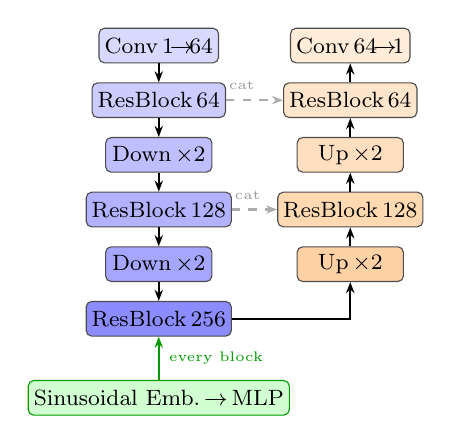
\begin{tikzpicture}[
    font=\footnotesize,
    block/.style={rectangle, rounded corners=2pt, draw=black!70,
                  fill=#1, minimum width=1.35cm, minimum height=0.44cm,
                  text centered, inner sep=2pt},
    temb/.style={rectangle, rounded corners=2pt, draw=green!60!black,
                 fill=green!18, minimum width=2.9cm, minimum height=0.44cm,
                 text centered, inner sep=2pt},
    arr/.style={-{Stealth[length=4pt]}, thick},
    skip/.style={-{Stealth[length=4pt]}, dashed, gray!65, thick},
    garr/.style={-{Stealth[length=4pt]}, green!60!black, thick},
    node distance=0.24cm and 0.9cm
  ]


  \node[block=blue!15]                   (in)  {Conv\,1$\!\to\!$64};
  \node[block=blue!20, below=of in]      (e1)  {ResBlock\,64};
  \node[block=blue!25, below=of e1]      (d1)  {Down\,$\times$2};
  \node[block=blue!30, below=of d1]      (e2)  {ResBlock\,128};
  \node[block=blue!35, below=of e2]      (d2)  {Down\,$\times$2};
  \node[block=blue!45, below=of d2]      (bot) {ResBlock\,256};

  \node[block=orange!15, right=0.9cm of in]  (out) {Conv\,64$\!\to\!$1};
  \node[block=orange!20, below=of out]       (de1) {ResBlock\,64};
  \node[block=orange!25, below=of de1]       (u1)  {Up\,$\times$2};
  \node[block=orange!30, below=of u1]        (de2) {ResBlock\,128};
  \node[block=orange!35, below=of de2]       (u2)  {Up\,$\times$2};


  \node[temb, below=0.55cm of bot] (te)
        {Sinusoidal Emb.\,$\to$\,MLP};

  \foreach \a/\b in {in/e1, e1/d1, d1/e2, e2/d2, d2/bot}
    \draw[arr] (\a) -- (\b);

  \draw[arr] (bot.east) -| (u2.south);

  \foreach \a/\b in {u2/de2, de2/u1, u1/de1, de1/out}
    \draw[arr] (\a) -- (\b);

  \draw[skip] (e1.east)  -| ++(0.2, 0) |- (de1.west)
        node[pos=0.25, above, gray!80, font=\tiny]{cat};
  \draw[skip] (e2.east)  -| ++(0.2, 0) |- (de2.west)
        node[pos=0.25, above, gray!80, font=\tiny]{cat};

  \draw[garr] (te.north) -- (bot.south)
        node[midway, right, font=\tiny, green!60!black]{every block};

\end{tikzpicture}
\caption{Residual U-Net architecture shared across all three model variants (FP16,
W1A16, W1A1). The encoder--decoder structure with channel widths [64,~128,~256],
skip connections (dashed, via concatenation), and sinusoidal time embedding injection
(green) is identical in all variants; only the convolution type changes (Conv2d /
BitConv2d\_Std / BitConv2d\_BNN).}
\label{fig:arch}
\end{figure}

\textbf{Time Conditioning.} Each diffusion step index is encoded with a 32-dimensional
sinusoidal embedding~\cite{vaswani2017attention} and then fed through a small two-layer
MLP, producing $t_\text{emb} \in \mathbb{R}^{32}$. Inside every residual block a
learned linear layer maps $t_\text{emb}$ to the block's channel count and adds it
element-wise to the feature map, so that timestep information is available at all
spatial resolutions.

\textbf{Boundary Layer Convention.} Following standard BNN practice, the input
convolution ($1{\to}64$ channels) and the output projection ($64{\to}1$ channels) remain
in full precision across all model variants. Keeping the pixel-space interface layers at
higher precision avoids introducing quantization noise at the boundaries of the network.

\subsection{Pre-Activation Block Structure}

Every binary residual block follows the pre-activation layout shown in
Figure~\ref{fig:block}. Written out, a single block computes:
\begin{align*}
  h &\leftarrow \text{BinaryAct}\!\left(\text{BN}(x)\right) \\
  h &\leftarrow \text{BinaryConv2d}(h) \\
  h &\leftarrow h + \text{Linear}(t_\text{emb}) \\
  h &\leftarrow \text{BinaryAct}\!\left(\text{BN}(h)\right) \\
  h &\leftarrow \text{BinaryConv2d}(h) \\
  \text{output} &\leftarrow h + \text{skip}(x)
\end{align*}

where \texttt{skip} is a 1$\times$1 BinaryConv2d when channel dimensions change, or an
identity otherwise.

\begin{figure}[t]
\centering

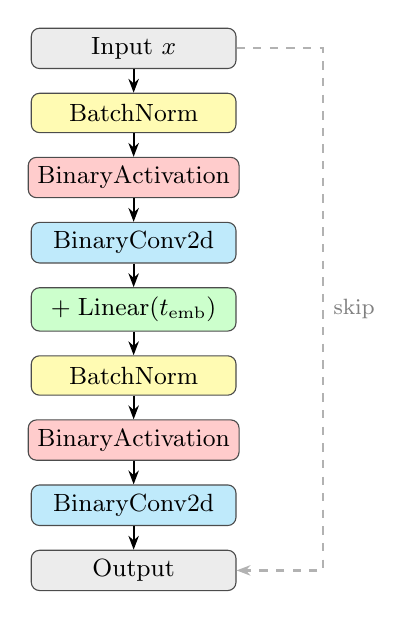
\begin{tikzpicture}[
    font=\small,
    op/.style={rectangle, rounded corners=3pt, draw=black!70,
               fill=#1, minimum width=2.6cm, minimum height=0.5cm,
               text centered},
    arr/.style={-{Stealth[length=5pt]}, thick},
    skip/.style={-{Stealth[length=5pt]}, dashed, gray!60, thick},
    node distance=0.3cm
  ]

  \node[op=gray!15]   (x)   {Input $x$};
  \node[op=yellow!30, below=of x]  (bn1) {BatchNorm};
  \node[op=red!20,    below=of bn1](ba1) {BinaryActivation};
  \node[op=cyan!25,   below=of ba1](bc1) {BinaryConv2d};
  \node[op=green!20,  below=of bc1](te)  {$+\;\text{Linear}(t_\text{emb})$};
  \node[op=yellow!30, below=of te] (bn2) {BatchNorm};
  \node[op=red!20,    below=of bn2](ba2) {BinaryActivation};
  \node[op=cyan!25,   below=of ba2](bc2) {BinaryConv2d};
  \node[op=gray!15,   below=of bc2](out) {Output};

  \foreach \a/\b in {x/bn1, bn1/ba1, ba1/bc1, bc1/te,
                     te/bn2, bn2/ba2, ba2/bc2, bc2/out}
    \draw[arr] (\a) -- (\b);

  \draw[skip] (x.east) -- ++(1.1,0) |- (out.east)
    node[pos=0.25, right, font=\footnotesize, gray]{skip};

\end{tikzpicture}
\caption{Pre-activation binary residual block. BatchNorm is applied \emph{before}
BinaryActivation at both sub-layers, ensuring sign-function inputs are
zero-centred throughout training (topological stability). The identity skip
connection preserves gradient flow to shallow layers.}
\label{fig:block}
\end{figure}

\textbf{Topological Stability via Pre-Activation Ordering.} What makes this ordering
important is that BatchNorm re-centres and re-scales activations \emph{before} they
reach the sign function.  Because the resulting distribution sits close to zero mean
with unit variance, the binary decision boundary stays well-calibrated at every
training iteration. Dead neurons and gradient starvation---two common failure modes when
sign functions are involved---are effectively avoided. We refer to this property as
\textbf{topological stability}: the binary representation stays dynamically balanced
enough to capture the class-level manifold boundaries of the data distribution,
sustaining diverse and structurally coherent generation.

\subsection{Mean-Centered Weight Binarization (Structural Dominance)}

Weight binarization in the W1A16 variant is handled by \texttt{BitConv2d\_Std}, a
convolution layer that subtracts the per-filter mean before applying the sign function.
Given a weight tensor $W \in \mathbb{R}^{C_\text{out} \times C_\text{in} \times k
\times k}$, let $w_o \in \mathbb{R}^{C_\text{in}k^2}$ denote the flattened kernel for
output channel $o$.

\textbf{Standard (uncentered) binarization:}
\begin{equation}
  \tilde{w}_o = \operatorname{sign}(w_o)\cdot\alpha_o,
  \quad
  \alpha_o = \frac{\|w_o\|_1}{C_\text{in}\cdot k^2}
  \label{eq:std-bin}
\end{equation}

\textbf{Centered binarization (\texttt{BitConv2d\_Std}):}
\begin{equation}
  \bar{w}_o = w_o - \mu_o,
  \quad
  \mu_o = \operatorname{mean}(w_o)
  \label{eq:center}
\end{equation}
\begin{equation}
  \hat{w}_o = \operatorname{sign}(\bar{w}_o)\cdot\bar\alpha_o,
  \quad
  \bar\alpha_o = \frac{\|\bar{w}_o\|_1}{C_\text{in}\cdot k^2}
  \label{eq:cen-bin}
\end{equation}

\textbf{Structural Dominance Property.} By subtracting $\mu_o$, the isotropic DC
component is stripped from the weight vector, leaving only its directional content
exposed. Applying the sign function then quantizes this purified direction, while
$\bar\alpha_o$ serves as a magnitude proxy that rescales the result. The key effect is
that $\hat{w}_o$ inherits the \emph{dominant directional structure} of the original
filter $w_o$: because a zero-mean vector's sign pattern faithfully reflects how its
entries are distributed across directions---unlike a vector biased by a large DC
offset---centering substantially shrinks the angular distortion that binarization
introduces. This property matters especially in diffusion networks, whose convolutional
kernels must capture oriented denoising responses in order to approximate the score
field accurately.

\subsection{Gradient Approximation via Straight-Through Estimator}

Both weight and activation binarization rely on the sign function, which has zero
derivative almost everywhere. To enable backpropagation through this hard threshold we
adopt the \textbf{Straight-Through Estimator}
(STE)~\cite{bengio2013ste}.

\textbf{Weight STE (\texttt{BitConv2d\_Std} and \texttt{BitConv2d\_BNN}):}
\begin{equation}
  w_\text{forward} = \underbrace{(\hat{w}_o - w_o)}_{\text{stop-grad}} + w_o
  \label{eq:ste-w}
\end{equation}

\textbf{Activation STE (W1A1 only, clipped):}
\begin{equation}
  \text{BinaryAct}(x) = \operatorname{sign}(x),
  \quad
  \frac{\partial\,\text{BinaryAct}}{\partial x} = \mathbf{1}[|x|\le 1]
  \label{eq:ste-a}
\end{equation}

Under the clipped variant~\cite{courbariaux2016clippedste}, gradients are set to zero
whenever $|x|>1$. This suppresses the destabilising influence of outlier activations
while keeping gradient information flowing through the bulk of the distribution.

\section{Experimental Setup}

\subsection{Model Architectures and Initialization}

Three model variants, all built on an identical U-Net backbone, are evaluated in our
experiments. Their configurations are summarized in Table~\ref{tab:variants}.

\begin{table}[h]
\centering
\caption{Model Variants}
\label{tab:variants}
\footnotesize
\begin{tabular}{@{}llll@{}}
\toprule
\textbf{Variant} & \textbf{Weights} & \textbf{Acts.} & \textbf{Key Layer} \\
\midrule
ResUNet\_FP16  & FP16              & FP16 (SiLU)        & Conv2d \\
ResUNet\_W1A16 & 1-bit, centered   & FP16 (SiLU)        & BitConv2d\_Std \\
ResUNet\_W1A1  & 1-bit, uncentered & 1-bit (clip.\ STE) & BitConv2d\_BNN \\
\bottomrule
\end{tabular}
\end{table}

Every model starts from PyTorch's default initialization. We train with the standard
DDPM objective under a linear noise schedule $\beta \in [10^{-4},\,0.02]$ spanning
$T=1{,}000$ diffusion steps. The FP16 and W1A16 variants are optimized with
Adam (lr $=10^{-3}$), while W1A1 uses
AdamW~\cite{loshchilov2019adamw} (lr $=10^{-4}$). All three are trained for 100 epochs
on the full MNIST~\cite{lecun1998mnist} training split (60{,}000 images, $28{\times}28$ grayscale, normalized
to $[-1,1]$) with a batch size of 16. The time-embedding MLP employs ReLU for FP16 and
W1A16 and GELU for W1A1. To ensure reproducibility, every reported metric is the mean
of three independent evaluation runs.

\subsection{The W1A16 Isolation Strategy}

Central to our experimental design is a \textbf{strict hardware ablation} in which
activation precision is held fixed at FP16 and only the weight binarization strategy
differs. By doing so, we decouple the binarization methodology (PTQ versus native) from
confounds introduced by activation quantization noise. The two variants under comparison
are:

\begin{itemize}
  \item \textbf{ResUNet\_W1A16 (Native):} Trained from scratch with
    \texttt{BitConv2d\_Std}.
  \item \textbf{ResUNet\_W1A16 (PTQ):} The trained FP16 model with weights post-hoc
    binarized via \texttt{BitConv2d\_Std}. Biases and BatchNorm statistics are
    preserved; only the convolutional weights are binarized.
\end{itemize}

Because activation precision is identical in both settings, any gap in generation quality
can be attributed directly to the training methodology---native versus post-training
binarization---rather than to differences in activation representation.

\subsection{Evaluation Metrics}

\textbf{Fr\'echet Inception Distance (FID).} We adopt FID~\cite{heusel2017fid}, which
quantifies the distance between two multivariate Gaussians fit to InceptionV3 features---one
from $N=2{,}000$ generated samples, the other from the MNIST test set. Before feature
extraction, all images are bilinearly upsampled from $28{\times}28$ to $299{\times}299$
and replicated across 3 channels:
\begin{equation}
  \text{FID} = \|\mu_r - \mu_g\|^2 +
  \operatorname{Tr}\!\left(\Sigma_r + \Sigma_g -
  2(\Sigma_r\Sigma_g)^{1/2}\right)
  \label{eq:fid}
\end{equation}

\textbf{Legibility Score.} As a task-specific probe for topological stability, we
introduce the Legibility Score: the average peak softmax confidence over $N=1{,}000$
generated images, evaluated by an MNISTClassifier trained separately on real data:
\begin{equation}
  \text{Legibility} = \frac{1}{N}\sum_{i=1}^{N}
  \max_{k\in\{0,\ldots,9\}} P\!\left(k \mid x_i^{\text{gen}}\right)
  \label{eq:legibility}
\end{equation}
Values close to 1.0 signal that the generator produces digits with strong class
commitment, whereas values around 0.10 (uniform chance) indicate manifold collapse.

\section{Results and Analysis}

\subsection{Quantitative Parity and Topological Stability}

The principal quantitative findings from the W1A16 hardware ablation appear in
Table~\ref{tab:main}.

\begin{table}[h]
\centering
\caption{Full Benchmark: Native vs.\ Post-Training Quantization}
\label{tab:main}
\begin{tabular}{@{}llcc@{}}
\toprule
\textbf{Model} & \textbf{Strategy} & \textbf{FID~$\downarrow$} &
\textbf{Legibility~$\uparrow$} \\
\midrule
ResUNet\_FP16  & Native (baseline) & $29.60 \pm 0.23$  & $90.79 \pm 0.51$\% \\
ResUNet\_W1A16 & \textbf{Native (ours)} & $\mathbf{24.24 \pm 1.15}$  & $\mathbf{89.45 \pm 0.73}$\% \\
ResUNet\_W1A16 & PTQ               & $191.94 \pm 1.37$ & $64.92 \pm 1.16$\% \\
\midrule
ResUNet\_W1A1  & \textbf{Native (ours)} & $\mathbf{83.98 \pm 1.66}$  & $\mathbf{81.02 \pm 0.54}$\% \\
ResUNet\_W1A1  & PTQ               & $223.00 \pm 1.89$ & $63.04 \pm 0.74$\% \\
\bottomrule
\end{tabular}
\end{table}

The outcome is unambiguous. With native training, the W1A16 model records FID~24.24 and
legibility~89.45\%, which not only matches but marginally \emph{exceeds} the FP16
baseline (FID~29.60, legibility~90.79\%). This indicates that the binary weight manifold
found through from-scratch training is no less expressive than its full-precision
counterpart on MNIST generation. PTQ, on the other hand, suffers a dramatic decline:
FID~191.94 ($7.9\times$ higher than the native model) with legibility falling to
64.92\%---evidence that retroactive binarization disrupts the learned score field,
although a degree of residual structure persists. Moving to the fully binary W1A1
regime, native training yields FID~83.98 and 81.02\% legibility, whereas PTQ decays
further to FID~223.00 and 63.04\% legibility. The W1A16 contrast is visualised in
Figure~\ref{fig:chart}.

\begin{figure}[h]
\centering
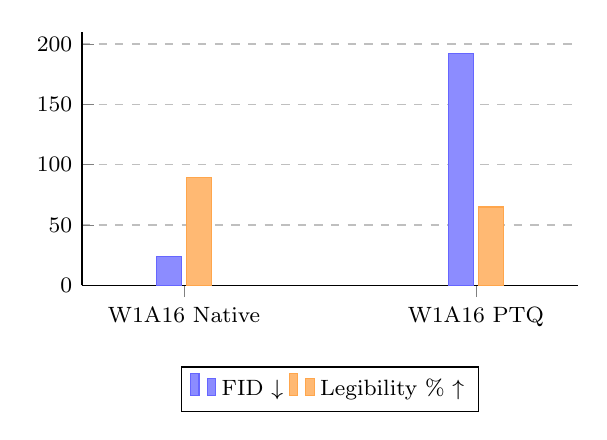
\begin{tikzpicture}
\begin{axis}[
    ybar,
    bar width=9pt,
    width=0.65\columnwidth,
    height=4.8cm,
    enlarge x limits=0.35,
    symbolic x coords={W1A16 Native, W1A16 PTQ},
    xtick=data,
    x tick label style={font=\footnotesize, align=center},
    ymin=0, ymax=210,
    ylabel style={font=\footnotesize},
    tick label style={font=\footnotesize},
    legend style={font=\footnotesize, at={(0.5,-0.32)}, anchor=north,
                  legend columns=2},
    axis y line*=left,
    axis x line*=bottom,
    ymajorgrids=true,
    grid style=dashed,
    clip=false,
    title style={font=\footnotesize\bfseries},
]

\addplot[fill=blue!45, draw=blue!60]
  coordinates {(W1A16 Native, 24.24) (W1A16 PTQ, 191.94)};
\addlegendentry{FID $\downarrow$};


\addplot[fill=orange!55, draw=orange!70]
  coordinates {(W1A16 Native, 89.45) (W1A16 PTQ, 64.92)};
\addlegendentry{Legibility \% $\uparrow$};
\end{axis}
\end{tikzpicture}
\caption{FID (lower is better, blue) and Legibility \% (higher is better, orange) for
the two W1A16 strategies. The native model attains markedly lower FID (24.24 vs.\
191.94) and higher legibility (89.45\% vs.\ 64.92\%) compared with PTQ. All values are
means across three independent runs.}
\label{fig:chart}
\end{figure}

\subsection{Visual Evidence of Quality Degradation}

Figures~\ref{fig:fp16}--\ref{fig:compare3way} supply visual corroboration of the
numerical results.

\begin{figure}[t]
  \centering
  \subfloat{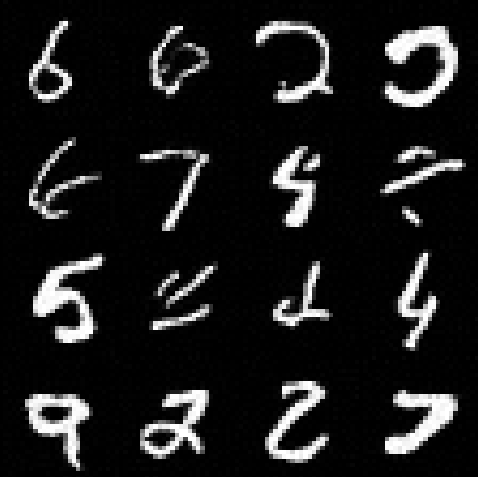
\includegraphics[width=0.35\columnwidth]{../assets/fp16_1.png}}\hfill
  \subfloat{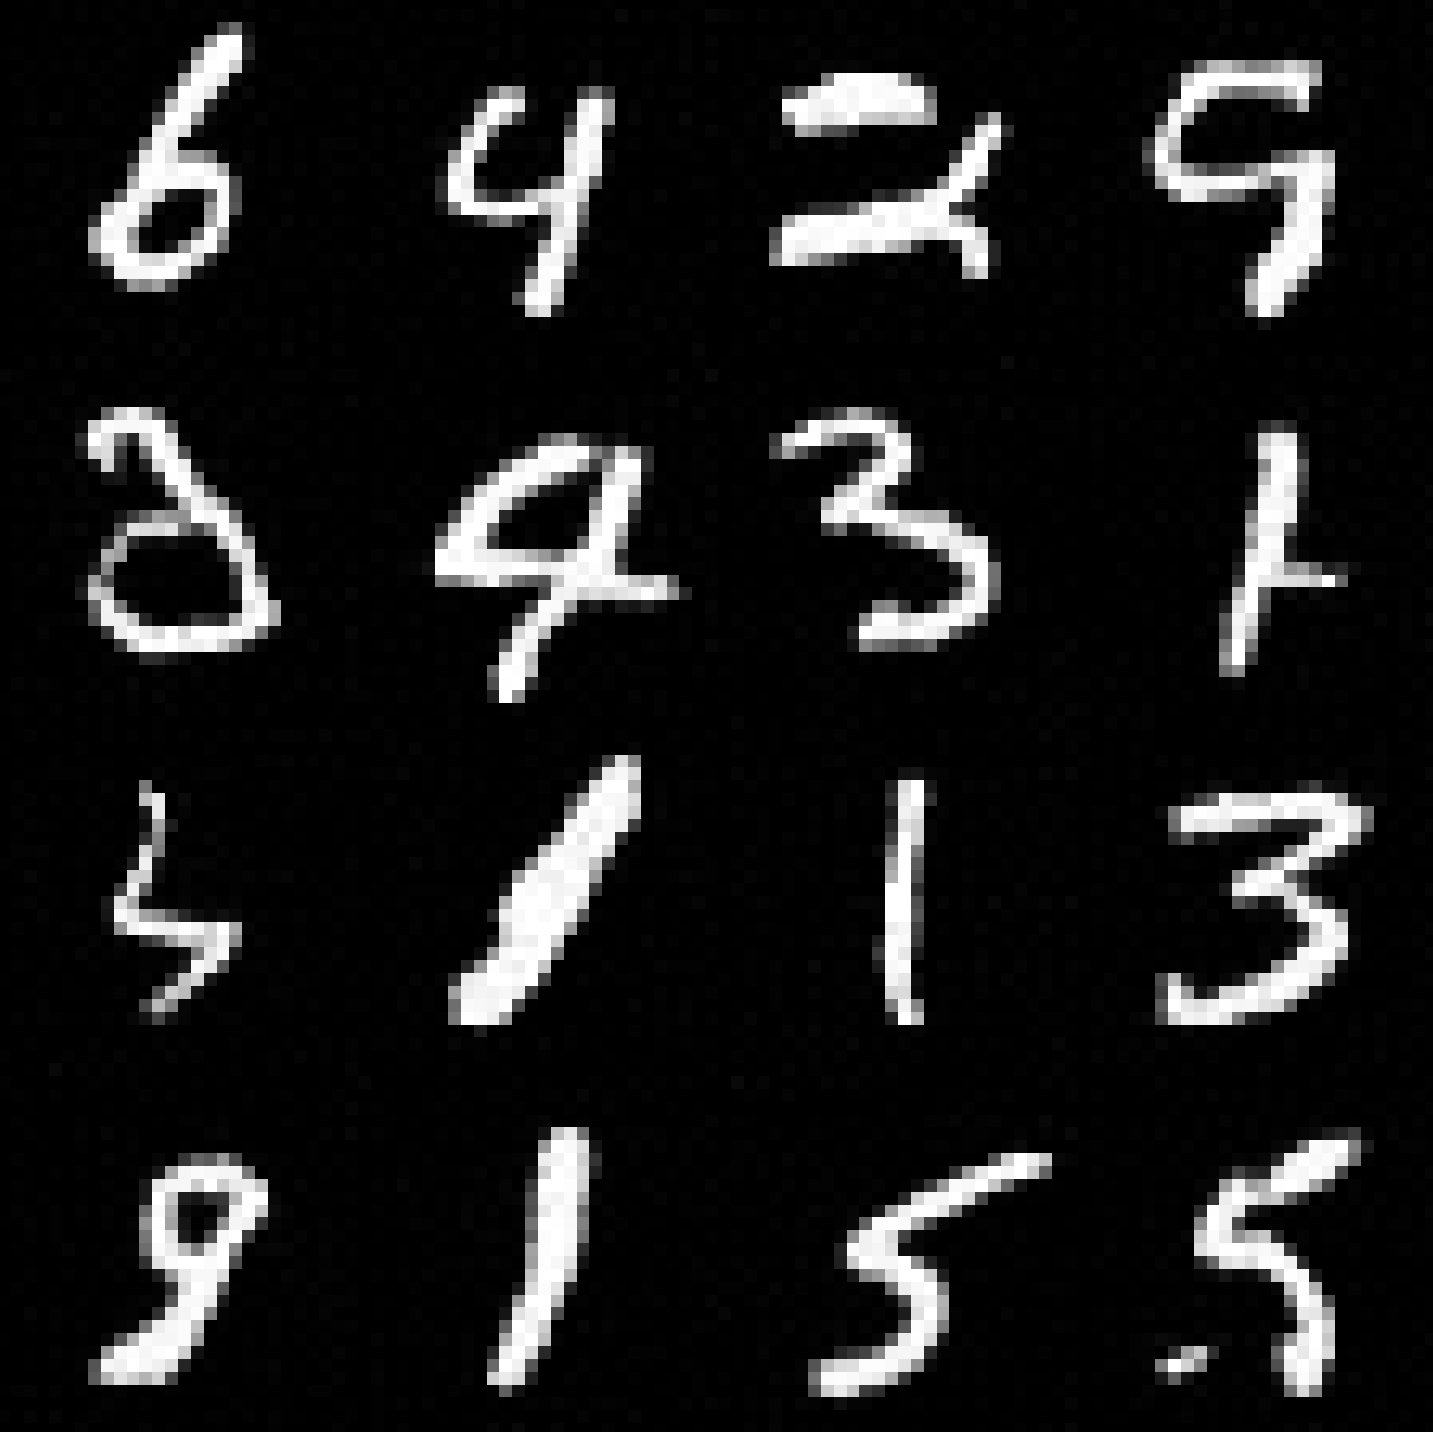
\includegraphics[width=0.35\columnwidth]{../assets/fp16_2.png}}
  \caption{ResUNet\_FP16 (full-precision baseline). Generated digits are crisp, varied,
  and clearly committed to individual classes---establishing the quality ceiling against
  which all compressed variants are compared.}
  \label{fig:fp16}
\end{figure}

\begin{figure}[t]
  \centering
  \subfloat{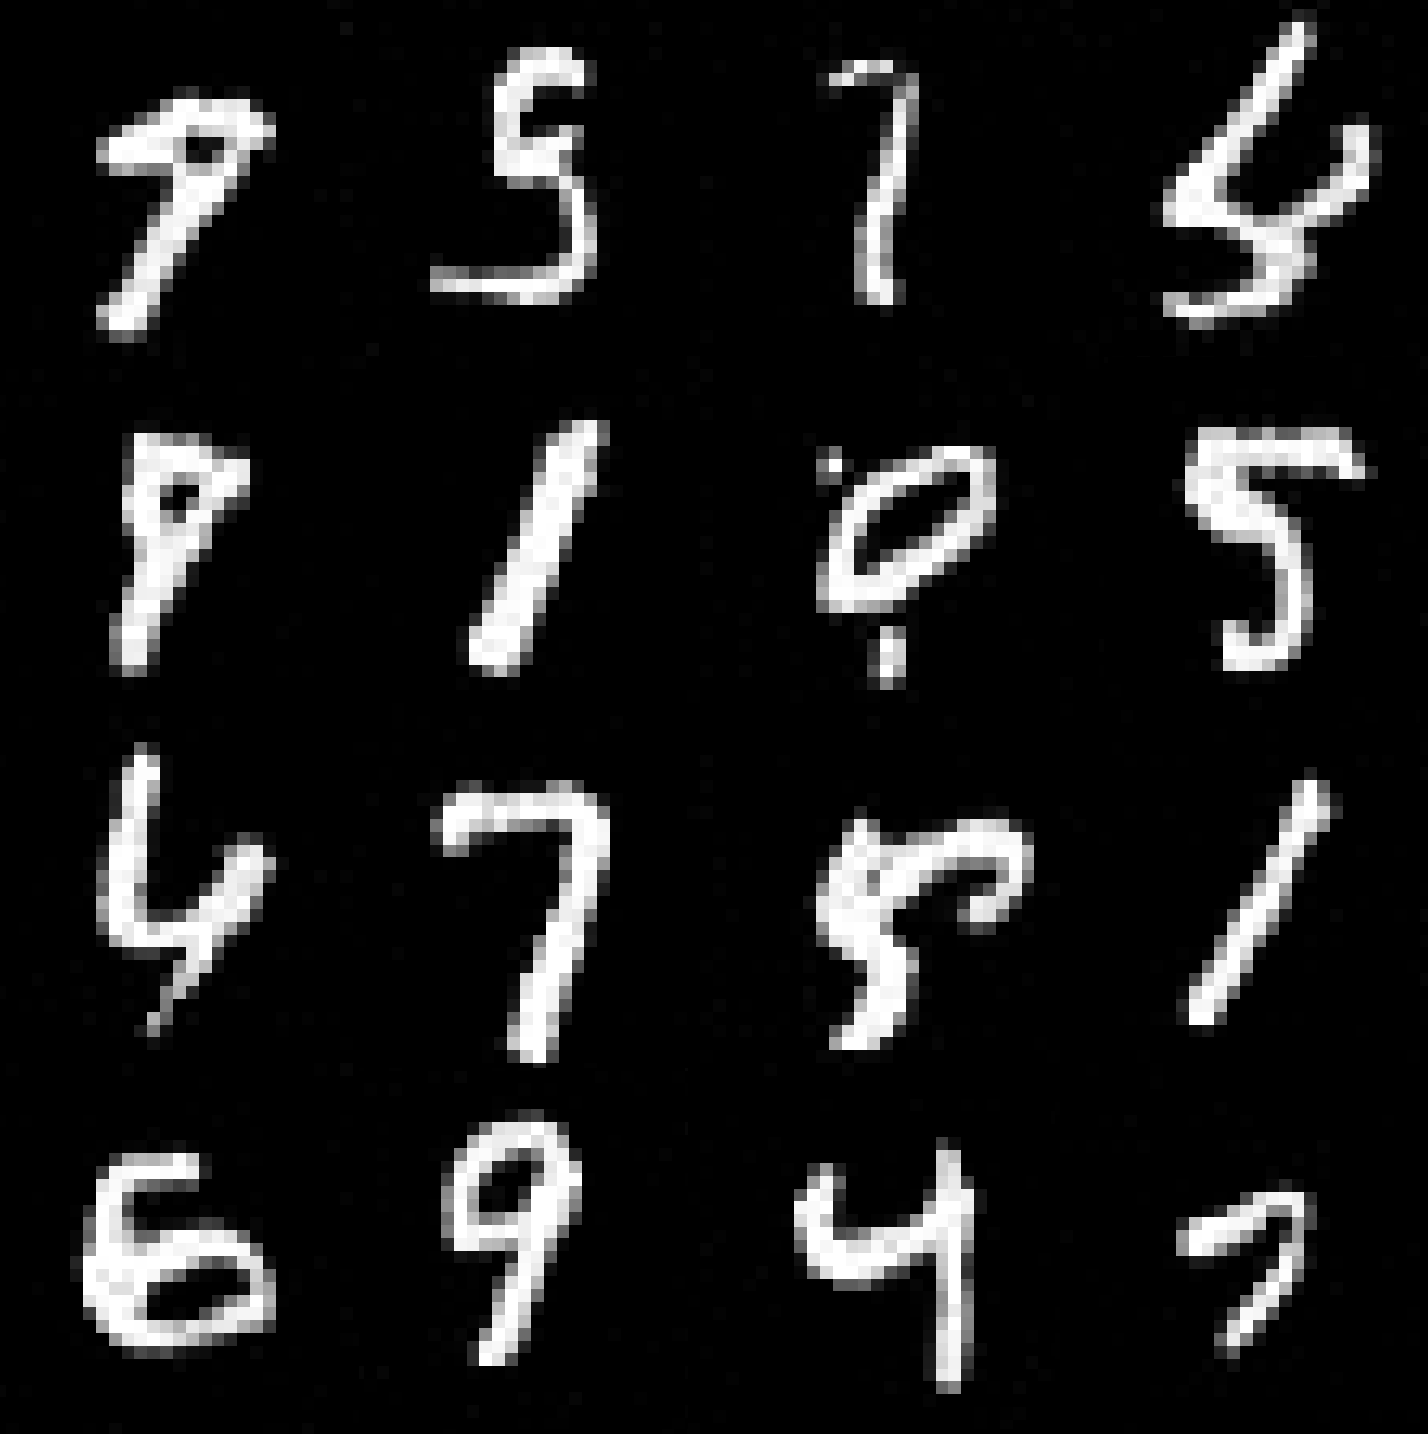
\includegraphics[width=0.35\columnwidth]{../assets/w1a16_our_output_1.png}}\hfill
  \subfloat{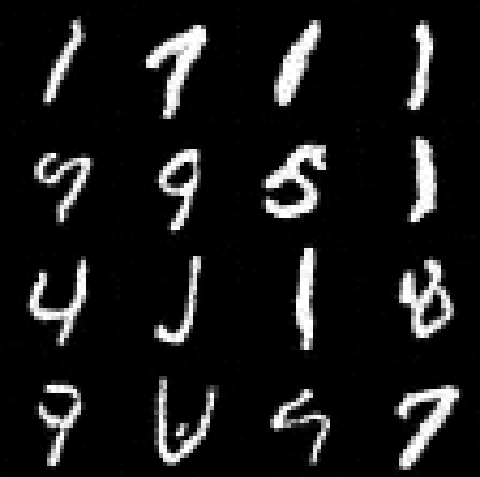
\includegraphics[width=0.35\columnwidth]{../assets/w1a16_our_output_2.png}}
  \caption{Natively trained ResUNet\_W1A16 (\textbf{structural dominance}: centered
  1-bit weights, FP16 activations). Both digit structure and class diversity remain
  visually intact, in line with the measured FID of 24.24 and 89.45\% legibility.}
  \label{fig:w1a16nat}
\end{figure}

\begin{figure}[t]
  \centering
  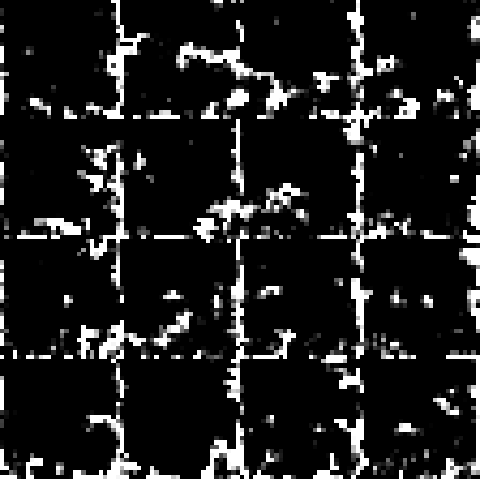
\includegraphics[width=0.45\columnwidth]{../assets/w1a16_quantized_1.png}
  \caption{PTQ ResUNet\_W1A16 (FP16 model binarized after training). Outputs exhibit
  pronounced structural degradation and diminished clarity, matching the measured
  FID of 191.94 and 64.92\% legibility---far below the native model, though some
  residual digit structure persists.}
  \label{fig:w1a16ptq}
\end{figure}

\begin{figure}[t]
  \centering
  \subfloat{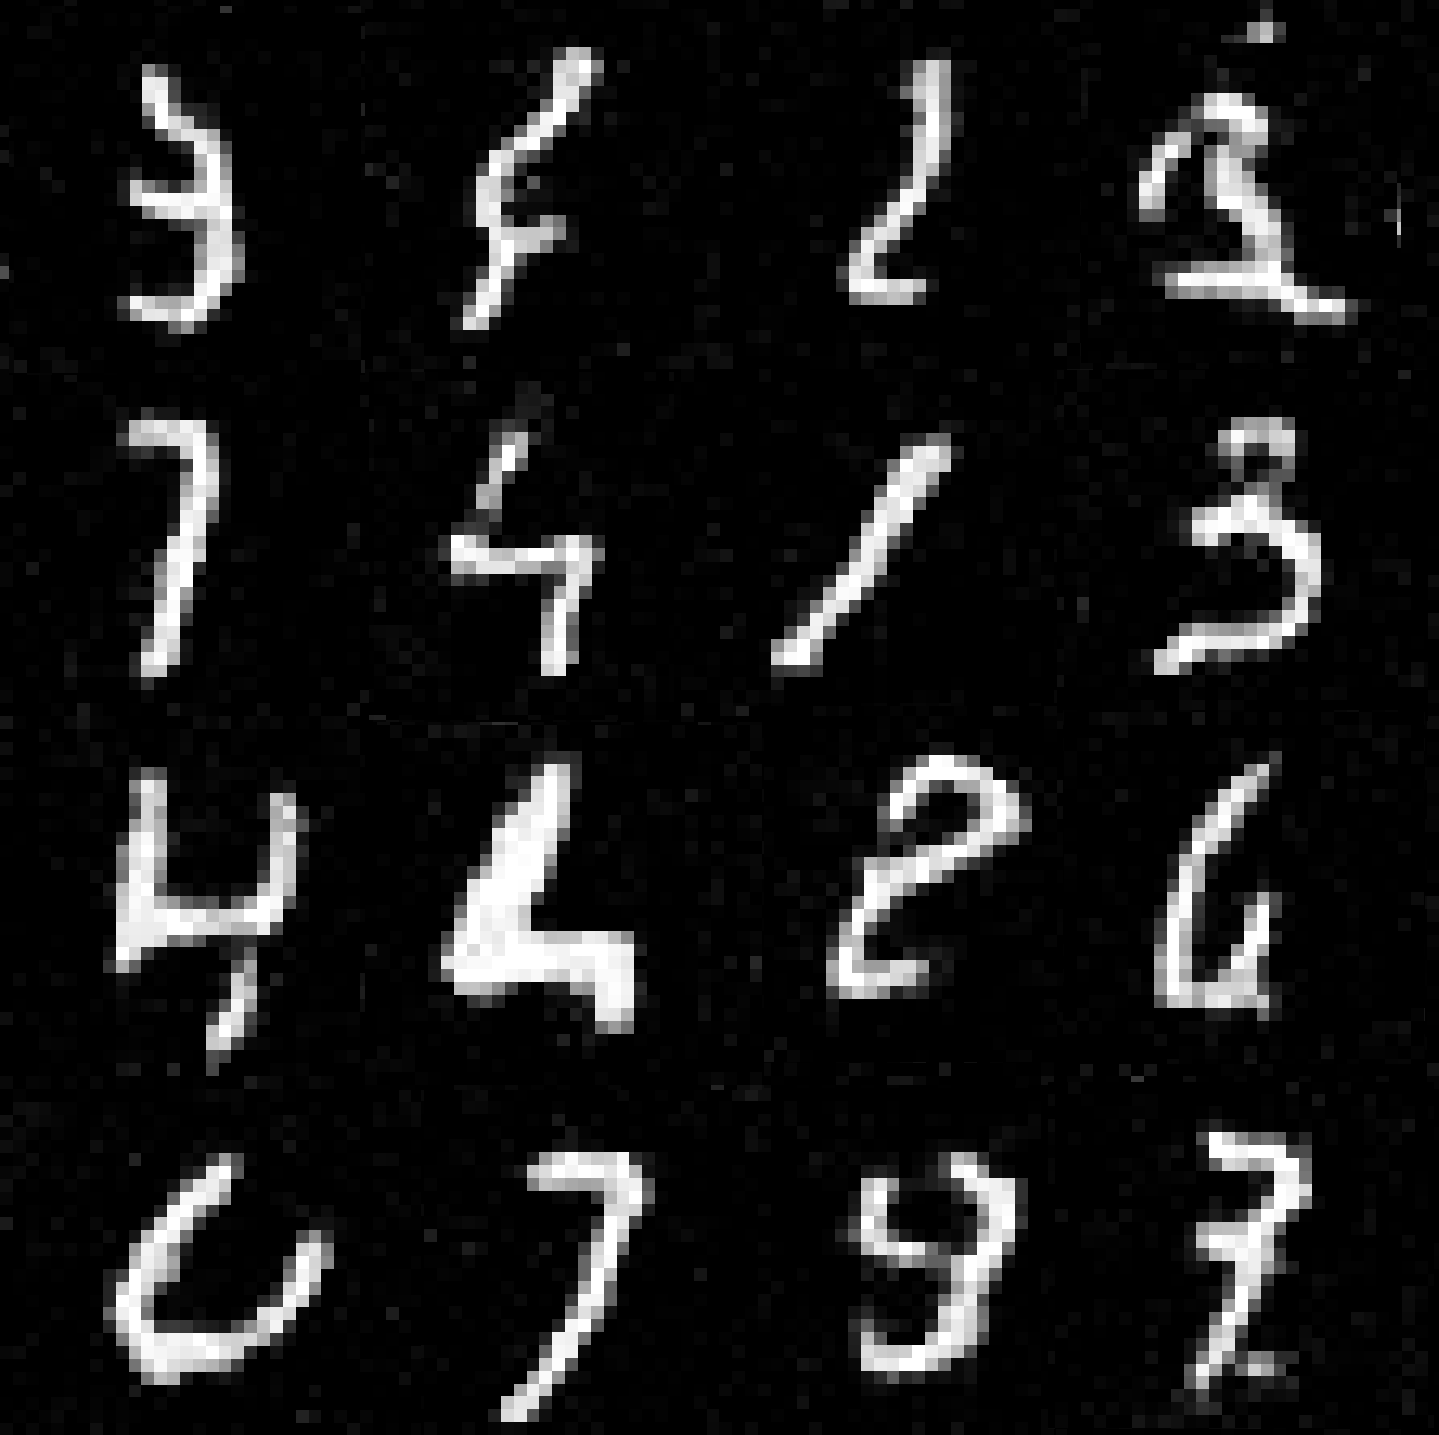
\includegraphics[width=0.35\columnwidth]{../assets/w1a1_our_output_1.png}}\hfill
  \subfloat{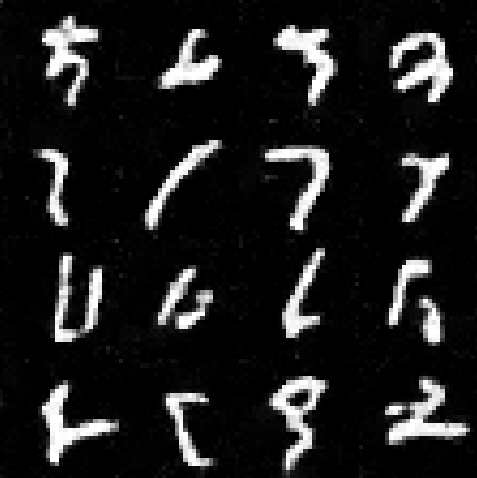
\includegraphics[width=0.35\columnwidth]{../assets/w1a1_our_output_2.png}}
  \caption{Natively trained ResUNet\_W1A1 (fully 1-bit: binary weights and binary
  activations, pre-activation ordering with clipped STE). Even under all-binary
  computation, digit topology is largely maintained---confirming that
  \textbf{topological stability} carries over to the fully binary setting.}
  \label{fig:w1a1nat}
\end{figure}

\begin{figure}[t]
  \centering
  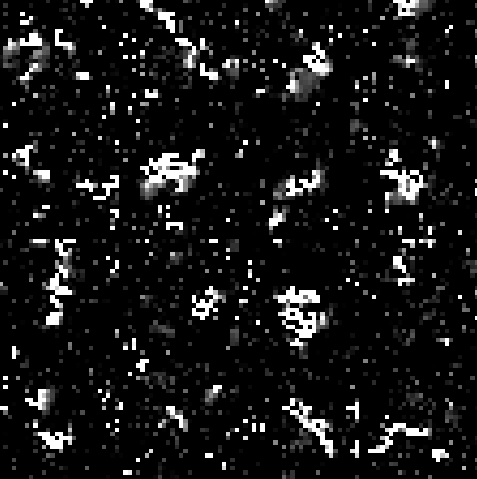
\includegraphics[width=0.45\columnwidth]{../assets/w1a1_quantized_1.png}
  \caption{PTQ ResUNet\_W1A1 (FP16 model fully binarized in both weights and activations).
  Activation binarization compounds the weight quantization error, producing additional
  structural degradation beyond that of PTQ W1A16 (Fig.~\ref{fig:w1a16ptq}).}
  \label{fig:w1a1ptq}
\end{figure}

\begin{figure}[t]
  \centering
  \subfloat[FP16]{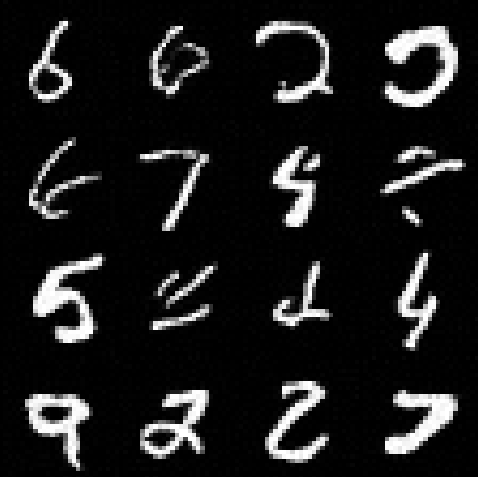
\includegraphics[width=0.22\columnwidth]{../assets/fp16_1.png}}\hfill
  \subfloat[W1A16 Native]{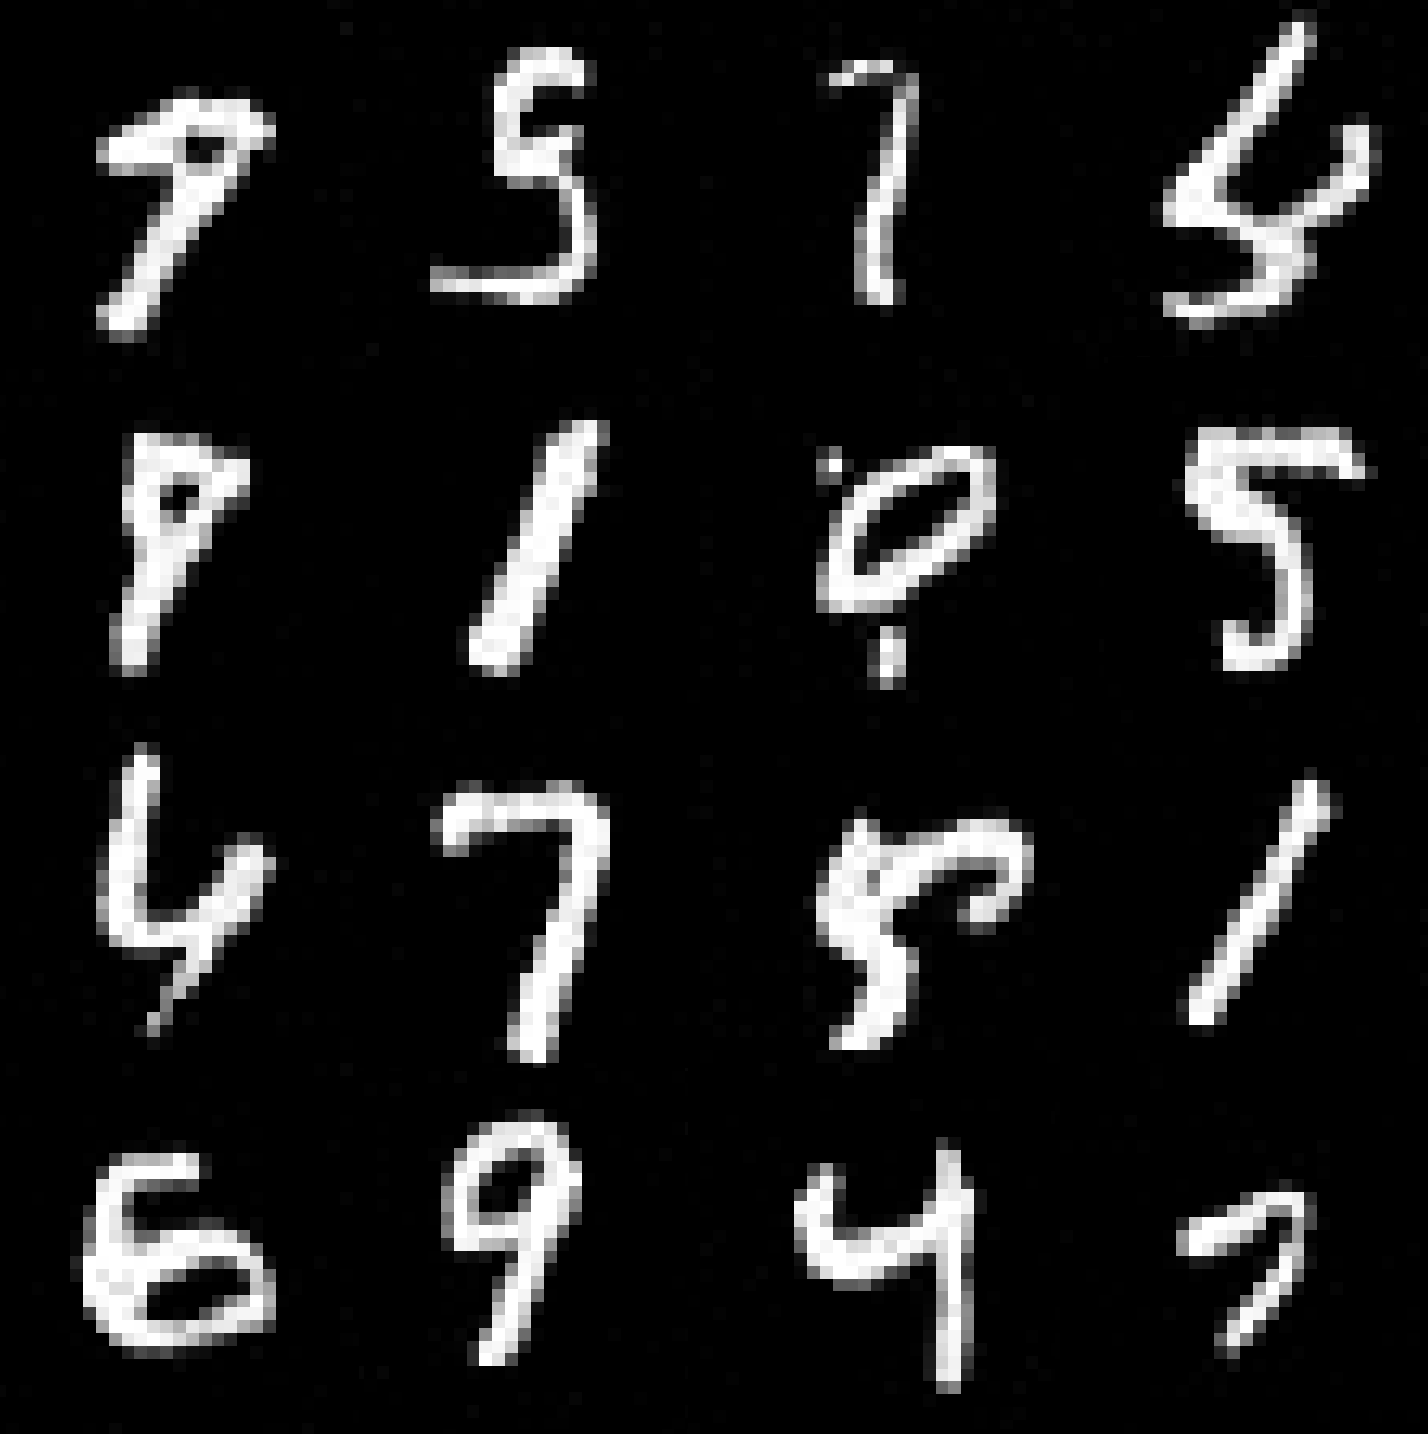
\includegraphics[width=0.22\columnwidth]{../assets/w1a16_our_output_1.png}}\hfill
  \subfloat[W1A1 Native]{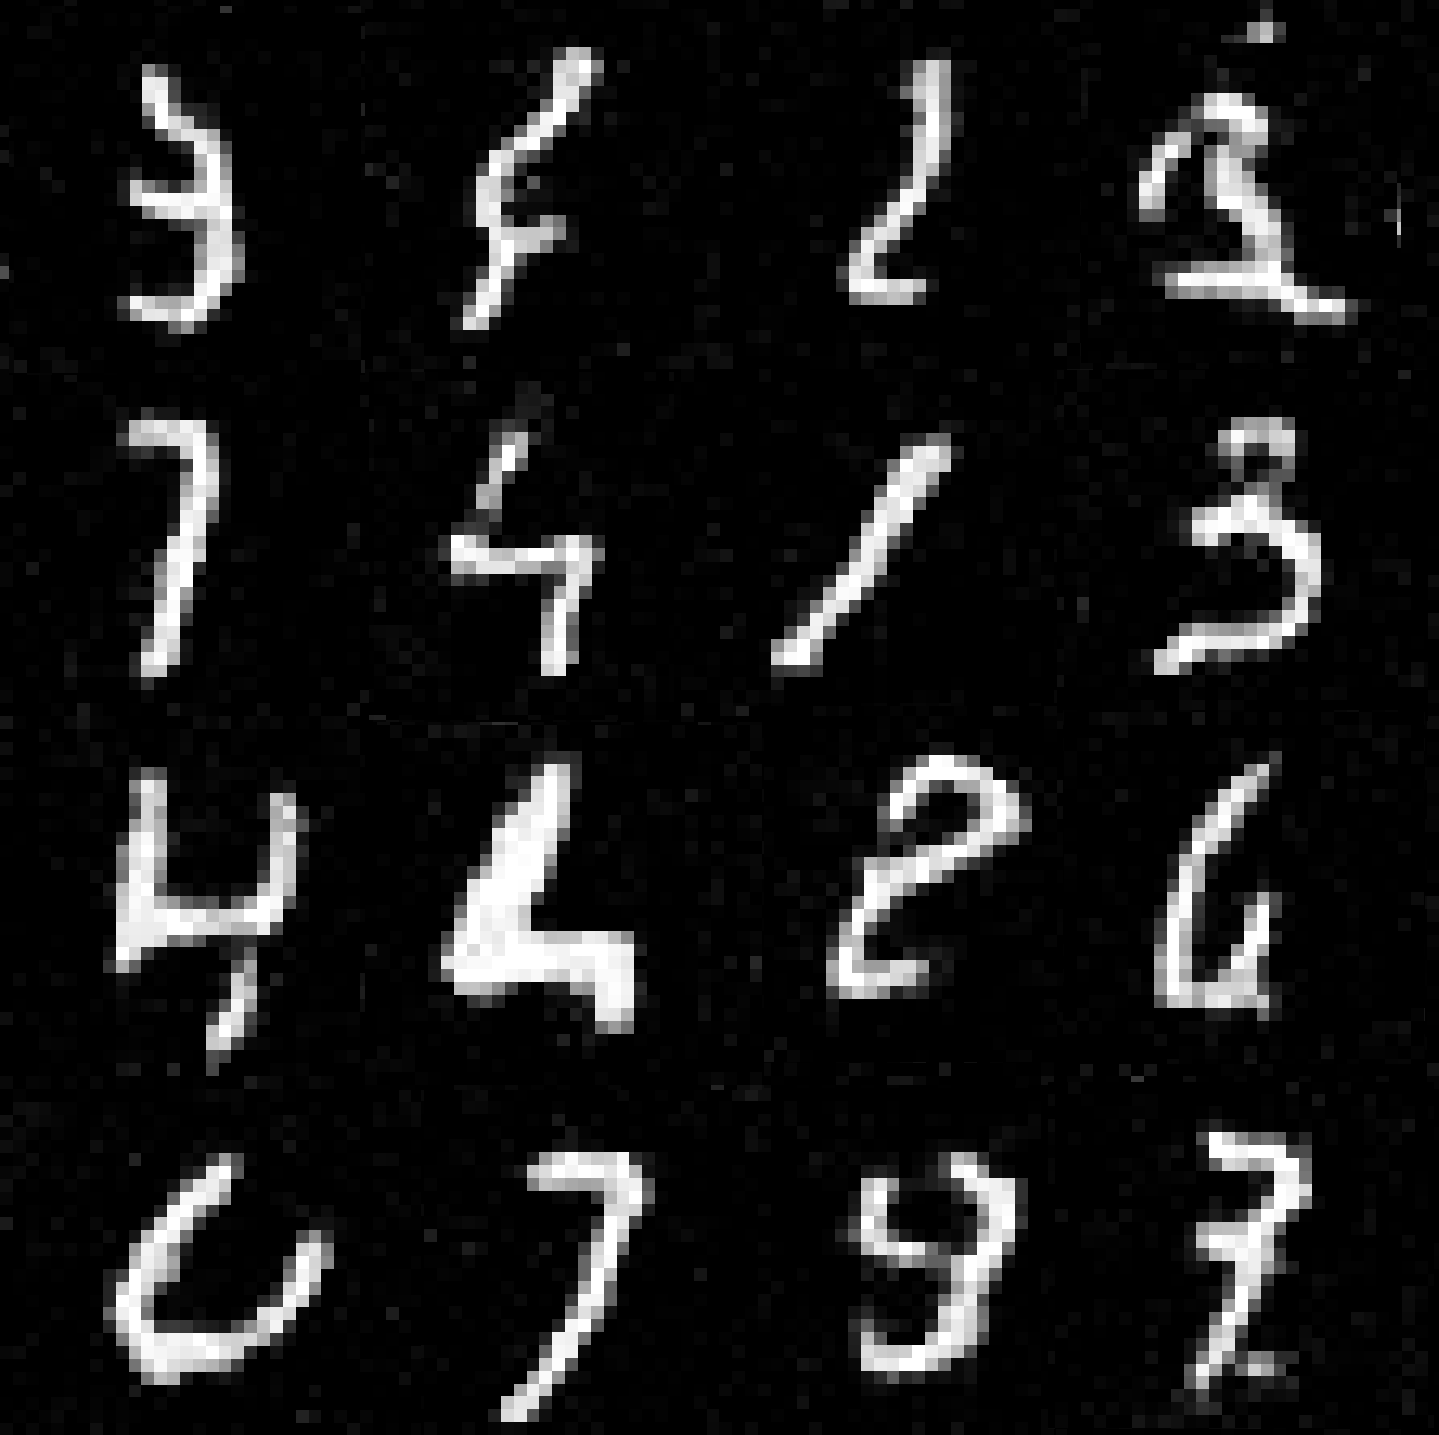
\includegraphics[width=0.22\columnwidth]{../assets/w1a1_our_output_1.png}}
  \caption{Three-way visual comparison. Quality degrades progressively, in keeping with
  the information-theoretic penalty of deeper quantization: the W1A16 native model
  preserves near-baseline fidelity, while W1A1 native exhibits the characteristic
  softening expected from the narrower representational bandwidth of fully binary
  activations.}
  \label{fig:compare3way}
\end{figure}

\subsection{Hardware Efficiency Gains}

Relative to ResUNet\_FP16, the W1A16 model offers the following theoretical hardware
advantages:

\begin{itemize}
  \item \textbf{Memory:} Each binarized convolutional weight requires only 1~bit,
    compared with 32~bits under FP32 storage---yielding a \textbf{32$\times$ memory
    reduction} across the binarized layers (16$\times$ relative to FP16 inference
    weights).
  \item \textbf{Arithmetic:} Multiplication with a binary weight reduces to a sign
    flip, implementable as an XNOR-popcount operation---a \textbf{58$\times$ reduction
    in binary operations} when measured against the FP16 MAC count (BOPs vs.\ FLOPs).
  \item \textbf{Energy:} On dedicated binary-arithmetic hardware, such operations
    draw roughly 1--2 orders of magnitude less energy than their floating-point
    counterparts.
\end{itemize}

Crucially, these savings come at \textbf{no measurable cost to semantic utility}: with
89.45\% legibility (compared to 90.79\% for FP16), the compressed model produces images
that are, at the digit-class level, semantically indistinguishable from those of the
full-precision baseline.

\section{Discussion}

\subsection{Why PTQ Fails at 1-Bit}

The structural dominance framework offers a clear mechanistic account of why PTQ
collapses at the 1-bit boundary. In a trained FP16 diffusion model, the score function
is encoded through the relative magnitudes and signs of filter weights together. Binary
quantization discards the entire magnitude ordering and keeps only the signs. Within a
converged FP16 network, however, individual weight signs carry negligible standalone
semantic content---information resides in the full magnitude-weighted interplay across
the filter. Extracting signs post-hoc therefore obliterates this encoding.

A second, complementary explanation is landscape-theoretic. The loss surfaces of the
DDPM objective under binary constraints and under full-precision parameterisation occupy
largely disjoint regions: the saddle points and minima reachable by $\{-1,+1\}$ weights
do not coincide with those of the FP16 model. PTQ projects the FP16 optimum onto the
binary parameter space, landing at a point that is neither optimal nor even stationary
under the binary loss. Native training, by contrast, explores the binary landscape from
the outset and converges to $\{-1,+1\}$ weight configurations that are genuine optima
of the DDPM objective within the binary constraint set.

\subsection{Structural Dominance vs.\ BiDM's Distillation}

BiDM~\cite{bidm2024} reports FID 22.74 on LSUN-Bedrooms $256{\times}256$ at W1A1
precision, relying on Timestep-friendly Binary Structure (TBS) together with Space
Patched Distillation (SPD). Their pipeline is inherently \emph{distillation-dependent}:
the binary student is trained to mimic the outputs of a full-precision teacher, creating
a hard dependency chain in which the binary model cannot be obtained without first
training the teacher it distils from. Native Binarization, in contrast, is
\emph{teacher-free}---the binary network discovers its own solution geometry
independently.

The practical ramifications of this difference are substantial. Whenever pre-trained
diffusion models are unavailable---as with custom medical imaging pipelines, proprietary
datasets, or entirely novel modalities---or when full-precision training is prohibitively
expensive or restricted by licensing, distillation-based routes become infeasible. Native
Binarization sidesteps this dependency altogether: only a single binary model needs to be
trained, cutting aggregate training cost and removing the storage burden of a teacher
checkpoint.

It is worth noting that the structural dominance principle---using centered weight
binarization to retain directional filter structure---is architecturally orthogonal to
BiDM's TBS and could, in principle, be incorporated into their learnable binarizer
framework to improve per-timestep binary weight fidelity.

\subsection{Topological Stability as a Generative Metric}

Legibility captures an aspect of generation quality that FID alone does not. FID rewards
both diversity and perceptual fidelity in feature space, yet it is blind to whether any
single sample is topologically committed to a particular class. A generator that produces
highly varied but structurally ambiguous digits could attain a moderate FID yet score
poorly on Legibility. Reporting both metrics together is therefore more revealing: FID
gauges how well the generator spans the full data distribution, while Legibility tests
whether each individual sample is a topologically coherent member of that distribution.

\subsection{Limitations}

Our experiments are limited to MNIST; scaling Native Binarization to higher-resolution
benchmarks such as CIFAR-10, CelebA, or LSUN-Bedrooms remains future work. The
Legibility Score depends on a task-specific classifier and does not transfer directly to
continuous-domain generation tasks. Additionally, the 58$\times$ operational speedup is
theoretical: realising it in practice demands specialised XNOR-popcount CUDA or FPGA
kernels, whereas our current code relies on standard PyTorch convolutions operating on
binary-valued weight tensors.

\section{Conclusion}

This paper introduced \textbf{Native Binarization}, a training framework for 1-bit
diffusion models built on two formally motivated principles: \textbf{structural
dominance} through mean-centered weight binarization, and \textbf{topological stability}
through pre-activation residual ordering. A controlled W1A16 hardware ablation revealed
that the sharp quality loss under standard PTQ (FID:~191.94, legibility:~64.92\%) is not
an intrinsic limitation of the 1-bit hardware boundary itself, but rather an artefact of
the Train-then-Quantize paradigm.

The natively trained W1A16 binary diffusion model achieves FID~24.24 and 89.45\%
legibility---effectively on par with the FP16 baseline (FID~29.60)---while delivering a
32$\times$ memory reduction and 58$\times$ computational speedup, all without
distilling knowledge from a full-precision teacher. These findings demonstrate that
1-bit diffusion manifolds are structurally viable when cultivated from scratch, and that
the structural dominance property of centered binarization supplies the inductive bias
needed for stable binary training.

We see Native Binarization as a concrete step toward teacher-free deployment of
aggressively compressed diffusion models on resource-limited edge devices. The structural
dominance and topological stability principles presented here are not architecture-specific
and may generalise to other generative families---flow matching models, consistency
models, and masked diffusion---wherever extreme 1-bit compression is desired without the
cost of maintaining a full-precision teacher.

\smallskip\noindent\textbf{Code Availability.} Source code and trained checkpoints are
publicly available at \url{https://github.com/nihal-gazi/Native-Binarization}.


\bibliographystyle{IEEEtran}
\bibliography{references}

\end{document}
